\newpage

\section{Data Mining}

This section presents the modeling process for fraud detection, including the implementation of multiple machine learning models, training strategies, evaluation metrics, and comparative analysis.

\subsection{Modeling Approach}

The objective is to classify transactions as fraudulent or non-fraudulent. The dataset is highly imbalanced, with a very small proportion of fraud cases. To address this issue, two training strategies were applied.

Two training strategies are considered:
\begin{itemize}
    \item \textbf{Imbalanced training}: using the original dataset, which reflects the real-world distribution but may bias models toward the majority class.
    
    \item \textbf{Balanced training (SMOTE)}: using an oversampled dataset to increase the representation of fraud cases, allowing models to better learn minority class patterns.
\end{itemize}

The following four models were selected for comparison:
\begin{itemize}
    \item \textbf{Logistic Regression}: A linear model used as a baseline. It is simple and interpretable, but may struggle with highly imbalanced data and non-linear relationships.
    
    \item \textbf{Decision Tree}: A non-linear model capable of capturing complex decision boundaries. However, it is prone to overfitting and may produce unstable results depending on the data distribution.
    
    \item \textbf{Gaussian Naive Bayes}: A probabilistic model based on the assumption of feature independence. This assumption is often unrealistic, which may limit its performance in real-world datasets.
    
    \item \textbf{Artificial Neural Network (MLP)}: A more powerful model that can learn complex non-linear relationships. It typically performs well with sufficient data but requires more computational resources and careful tuning.
\end{itemize}
These models were chosen for their diversity and uniqueness in learning mechanisms. Importantly, we wanted to compare or evaluate their effectiveness on this specific fraud detection problem.


Each model is trained on both datasets, and predictions are evaluated on validation and test sets. The predicted probabilities are converted into class labels using a threshold:
\[
y_{\text{pred}} = (y_{\text{prob}} \geq \text{threshold})
\]

Three thresholds are examined:

\begin{itemize}
    \item \textbf{Threshold = 0.7}: prioritizes precision (fewer false positives)
    \item \textbf{Threshold = 0.5}: standard default setting
    \item \textbf{Threshold = 0.2}: prioritizes recall (fewer missed fraud cases)
\end{itemize}
This experimentation allows evaluating how the trade-off between precision and recall changes under different decision thresholds.



\subsection{Evaluation Metrics}

The models were evaluated using the following metrics:

\begin{itemize}
    \item \textbf{Accuracy}: overall correctness of predictions
    \item \textbf{Precision}: proportion of predicted fraud cases that are actually fraud
    \item \textbf{Recall}: proportion of actual fraud cases correctly detected
    \item \textbf{F1-score}: harmonic mean of precision and recall
    \item \textbf{ROC-AUC}: ability to distinguish between classes
    \item \textbf{PR-AUC}: performance on imbalanced data
\end{itemize}

Among these, \textbf{Recall} and \textbf{PR-AUC} are the most important due to the imbalanced nature of the dataset.



\subsection{Results}

\paragraph*{Threshold = 0.7}

\begin{table}[H]
\centering
\small
\begin{tabular}{llcccccc}
\hline
Train & Model & Acc & Prec & Rec & F1 & ROC-AUC & PR-AUC \\
\hline
balanced & ANN\_MLP & 0.9907 & 0.3768 & 0.8719 & 0.5262 & 0.9898 & 0.8258 \\
balanced & DecisionTree & 0.9733 & 0.1683 & 0.8888 & 0.2830 & 0.9716 & 0.6556 \\
balanced & BayesianNB & 0.9359 & 0.0594 & 0.6612 & 0.1090 & 0.8428 & 0.2309 \\
balanced & LogisticReg & 0.9779 & 0.1667 & 0.6821 & 0.2680 & 0.8816 & 0.1939 \\
\hline
imbalanced & ANN\_MLP & 0.9980 & 0.9543 & 0.6918 & 0.8021 & 0.9925 & 0.8652 \\
imbalanced & DecisionTree & 0.9850 & 0.2770 & 0.9454 & 0.4284 & 0.9732 & 0.8315 \\
imbalanced & LogisticReg & 0.9765 & 0.1632 & 0.7191 & 0.2661 & 0.8942 & 0.2050 \\
imbalanced & BayesianNB & 0.9800 & 0.1500 & 0.5098 & 0.2318 & 0.8679 & 0.1636 \\
\hline
\end{tabular}
\caption{Model performance with threshold = 0.7}
\end{table}

\paragraph*{Threshold = 0.5}

\begin{table}[H]
\centering
\small
\begin{tabular}{llcccccc}
\hline
Train & Model & Acc & Prec & Rec & F1 & ROC-AUC & PR-AUC \\
\hline
balanced & ANN\_MLP & 0.9871 & 0.2995 & 0.8830 & 0.4473 & 0.9898 & 0.8258 \\
balanced & DecisionTree & 0.9580 & 0.1156 & 0.9135 & 0.2052 & 0.9716 & 0.6556 \\
balanced & BayesianNB & 0.8826 & 0.0350 & 0.7081 & 0.0668 & 0.8428 & 0.2309 \\
balanced & LogisticReg & 0.9169 & 0.0529 & 0.7692 & 0.0990 & 0.8816 & 0.1939 \\
\hline
imbalanced & ANN\_MLP & 0.9981 & 0.9172 & 0.7419 & 0.8203 & 0.9925 & 0.8652 \\
imbalanced & DecisionTree & 0.9830 & 0.2522 & 0.9480 & 0.3985 & 0.9732 & 0.8315 \\
imbalanced & LogisticReg & 0.9350 & 0.0681 & 0.7861 & 0.1254 & 0.8942 & 0.2050 \\
imbalanced & BayesianNB & 0.9765 & 0.1298 & 0.5202 & 0.2078 & 0.8679 & 0.1636 \\
\hline
\end{tabular}
\caption{Model performance with threshold = 0.5}
\end{table}

\paragraph*{Threshold = 0.2}

\begin{table}[H]
\centering
\small
\begin{tabular}{llcccccc}
\hline
Train & Model & Acc & Prec & Rec & F1 & ROC-AUC & PR-AUC \\
\hline
balanced & ANN\_MLP & 0.9785 & 0.2051 & 0.9122 & 0.3349 & 0.9898 & 0.8258 \\
balanced & DecisionTree & 0.9382 & 0.0825 & 0.9317 & 0.1516 & 0.9716 & 0.6556 \\
balanced & BayesianNB & 0.5552 & 0.0111 & 0.8420 & 0.0220 & 0.8428 & 0.2309 \\
balanced & LogisticReg & 0.4042 & 0.0090 & 0.9129 & 0.0178 & 0.8816 & 0.1939 \\
\hline
imbalanced & ANN\_MLP & 0.9977 & 0.8126 & 0.8062 & 0.8094 & 0.9925 & 0.8652 \\
imbalanced & DecisionTree & 0.9805 & 0.2268 & \textbf{0.9493} & 0.3661 & 0.9732 & 0.8315 \\
imbalanced & LogisticReg & 0.3941 & 0.0089 & 0.9161 & 0.0176 & 0.8942 & 0.2050 \\
imbalanced & BayesianNB & 0.9709 & 0.1077 & 0.5371 & 0.1794 & 0.8679 & 0.1636 \\
\hline
\end{tabular}
\caption{Model performance with threshold = 0.2}
\end{table}



\subsection{Visualization}

This subsection presents visualizations to better understand model performance under different training strategies and evaluation perspectives.

\paragraph*{Confusion Matrices}

\begin{figure}[H]
    \centering
    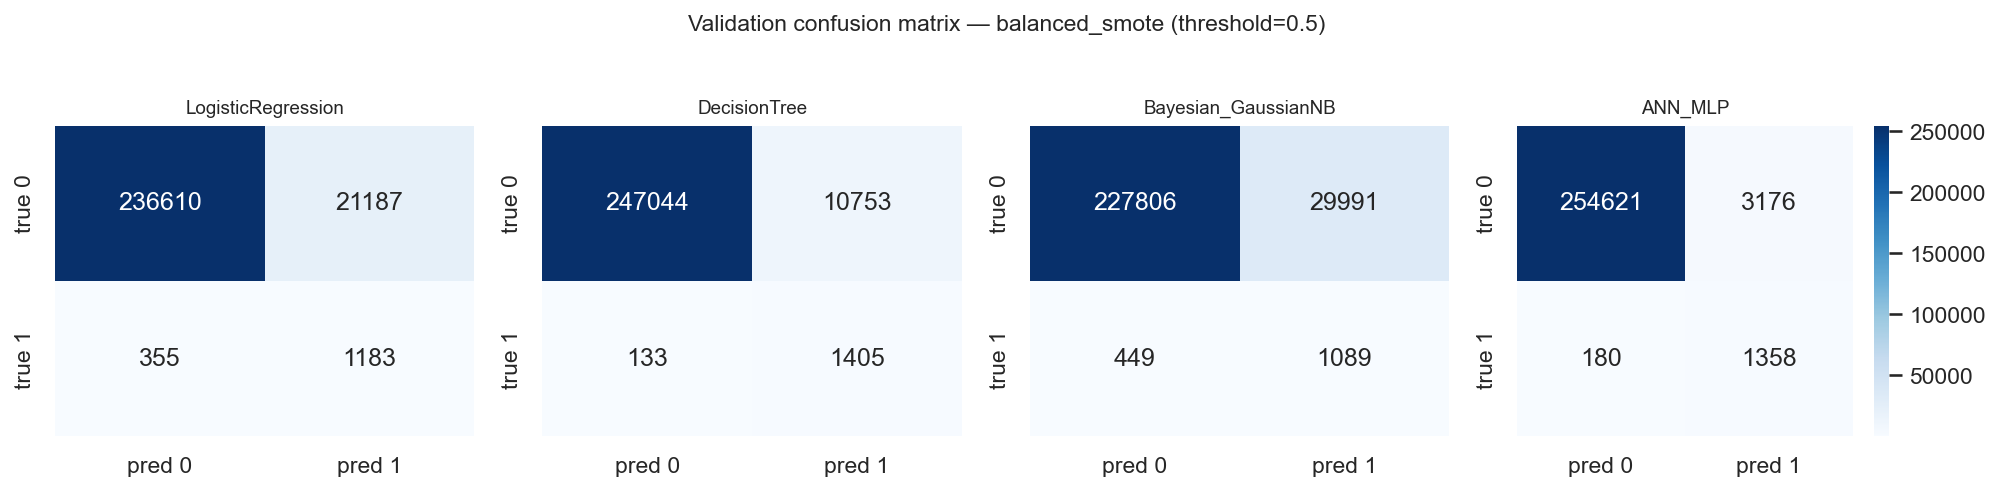
\includegraphics[width=1\textwidth]{Images/confusion_valid_balanced_smote_threshold_0.5.png}
    \caption{Confusion matrix on validation set (SMOTE, threshold = 0.5)}
    \label{fig:confusion_valid_smote}
\end{figure}

\begin{figure}[H]
    \centering
    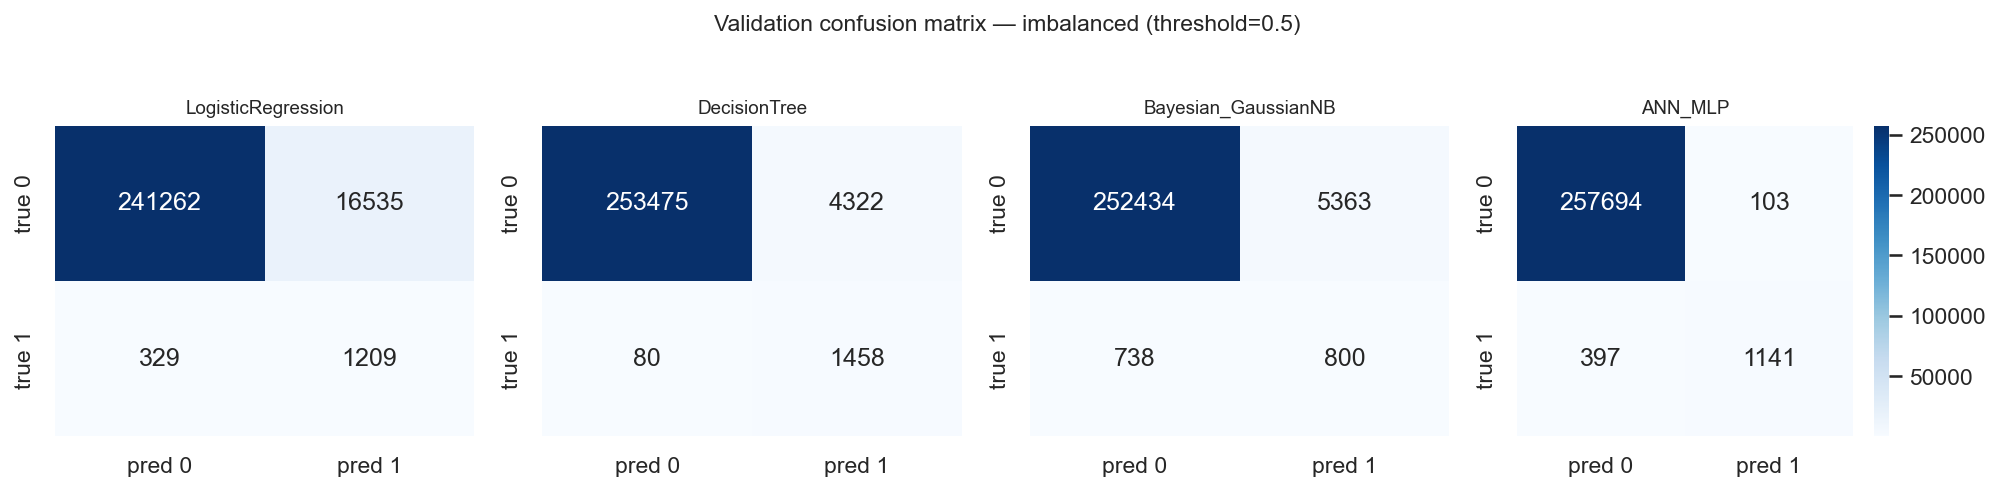
\includegraphics[width=1\textwidth]{Images/confusion_valid_imbalanced_threshold_0.5.png}
    \caption{Confusion matrix on validation set (imbalanced, threshold = 0.5)}
    \label{fig:confusion_valid_imbalanced}
\end{figure}

The confusion matrices illustrate the trade-off between detecting fraudulent transactions and avoiding false positives.

\paragraph*{Metric Comparison}

\begin{figure}[H]
    \centering
    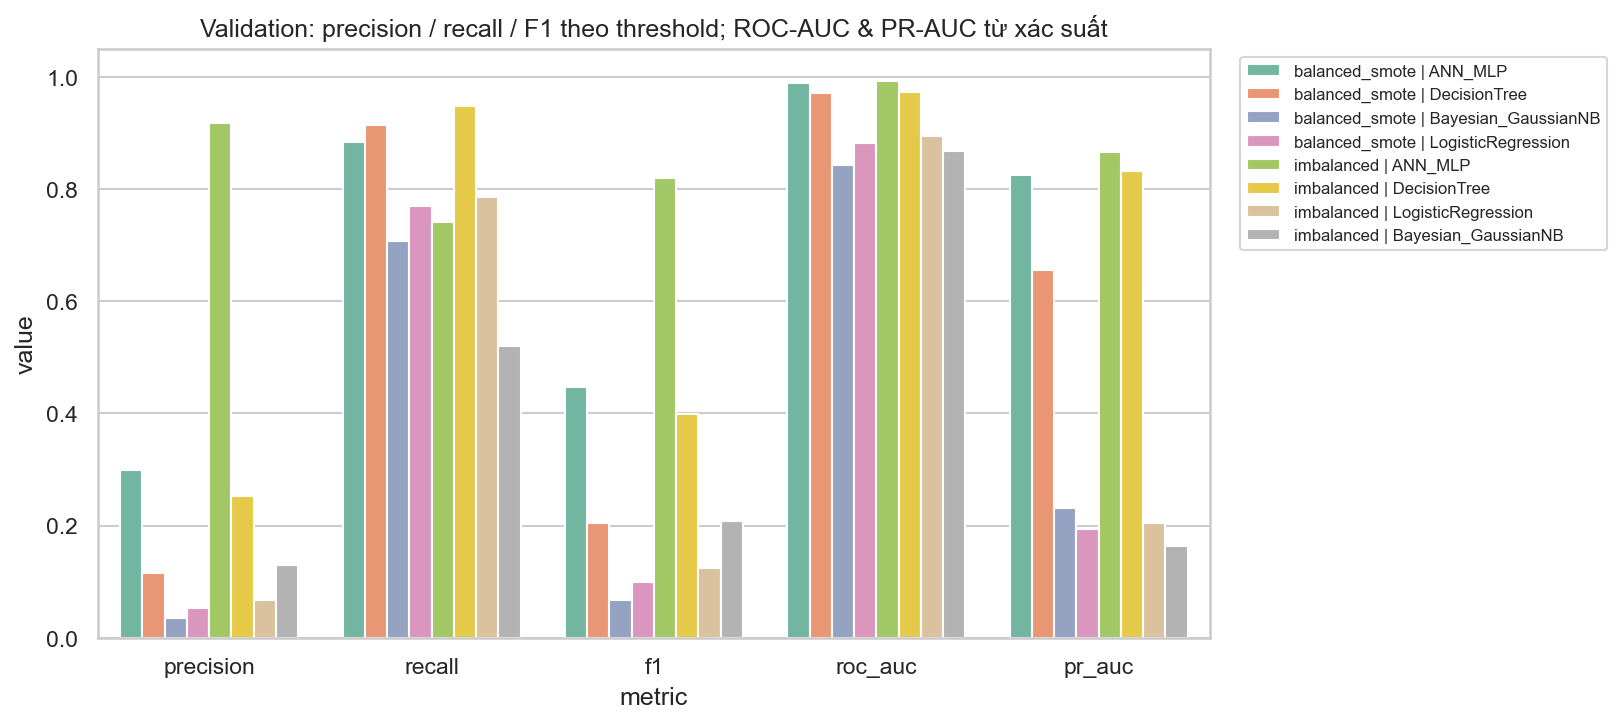
\includegraphics[width=1\textwidth]{Images/metrics_bar_valid_threshold_0.5.png}
    \caption{Metric comparison on validation set (threshold = 0.5)}
    \label{fig:metrics_valid}
\end{figure}

\begin{figure}[H]
    \centering
    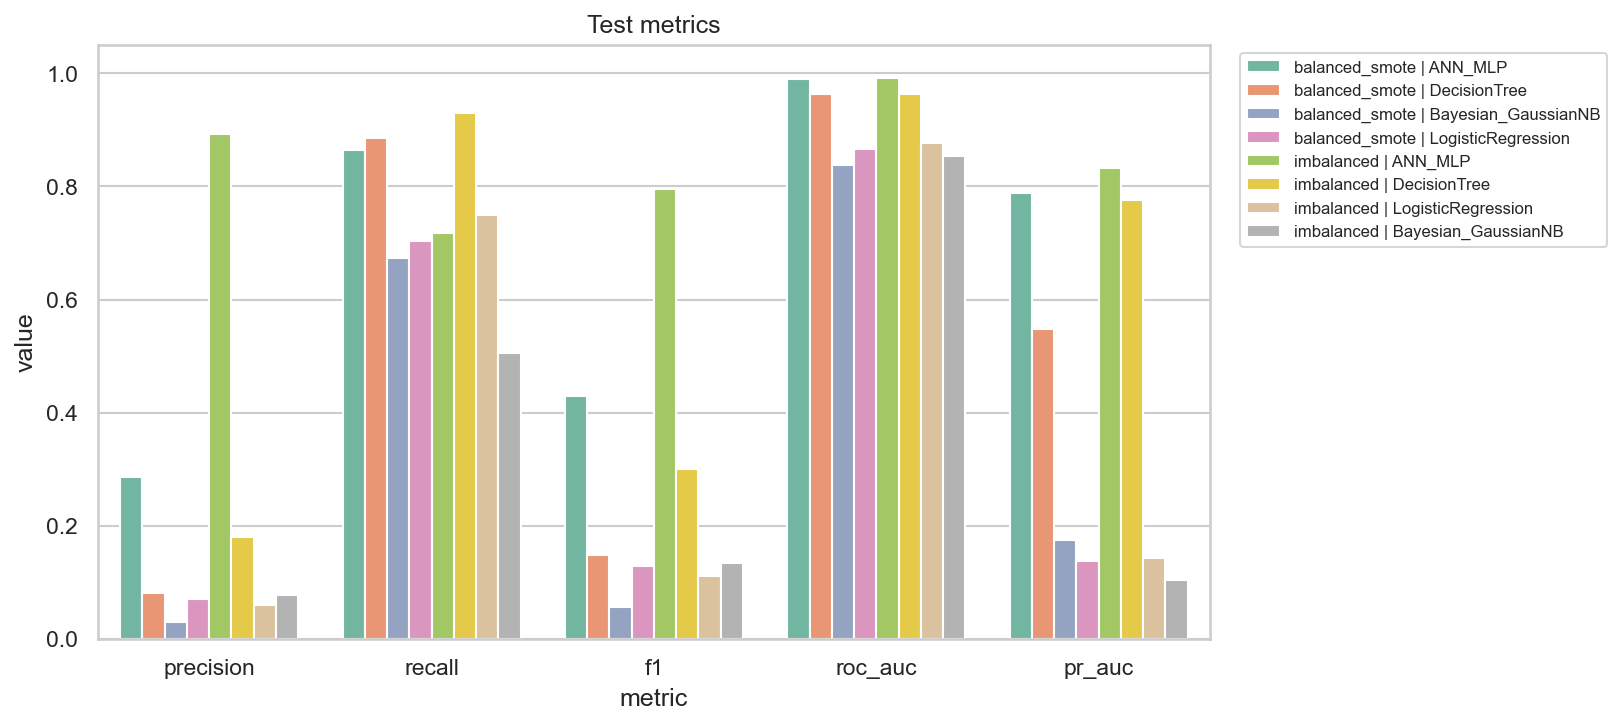
\includegraphics[width=1\textwidth]{Images/metrics_bar_test_threshold_0.5.png}
    \caption{Metric comparison on test set (threshold = 0.5)}
    \label{fig:metrics_test}
\end{figure}

\paragraph*{Precision-Recall Curves}

\begin{figure}[H]
    \centering
    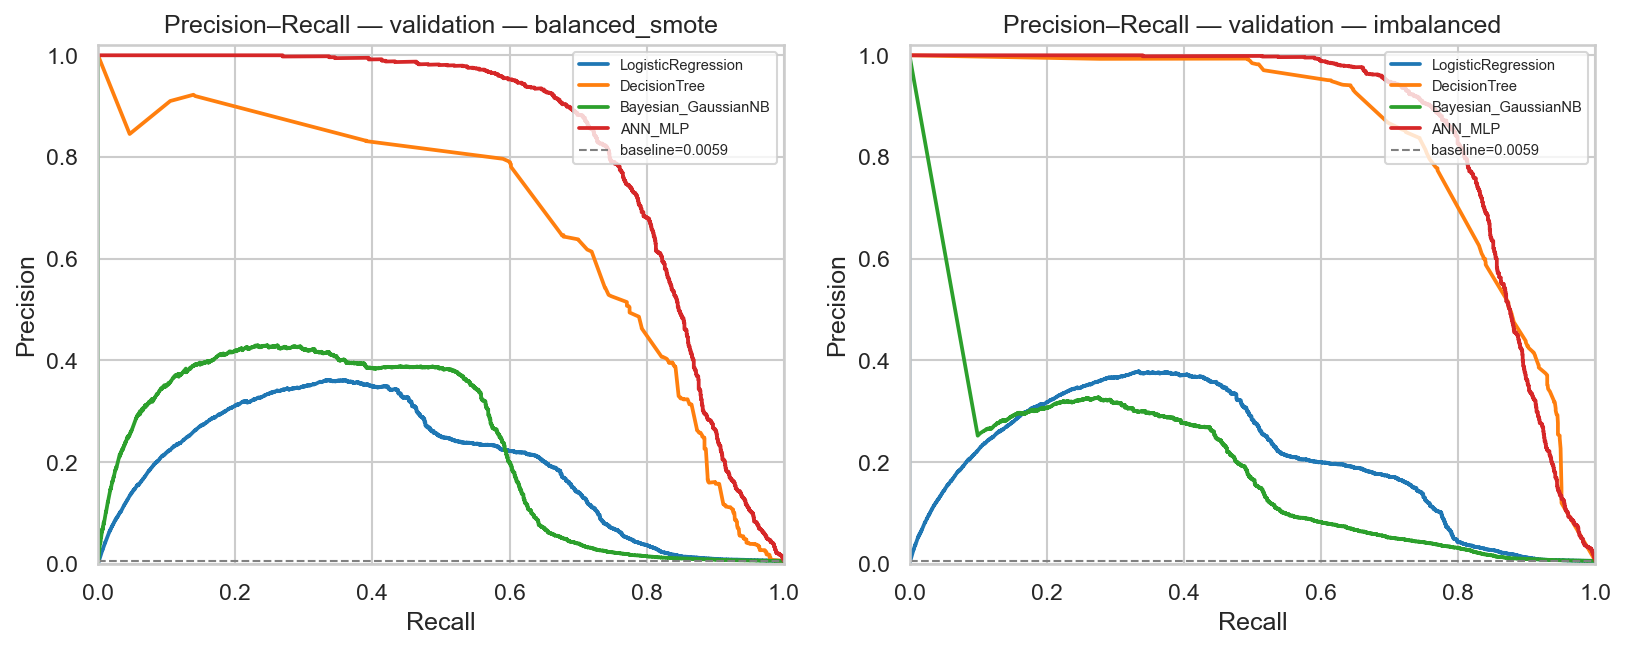
\includegraphics[width=1\textwidth]{Images/pr_valid_threshold_0.5.png}
    \caption{Precision-Recall curve on validation set}
    \label{fig:pr_valid}
\end{figure}

\begin{figure}[H]
    \centering
    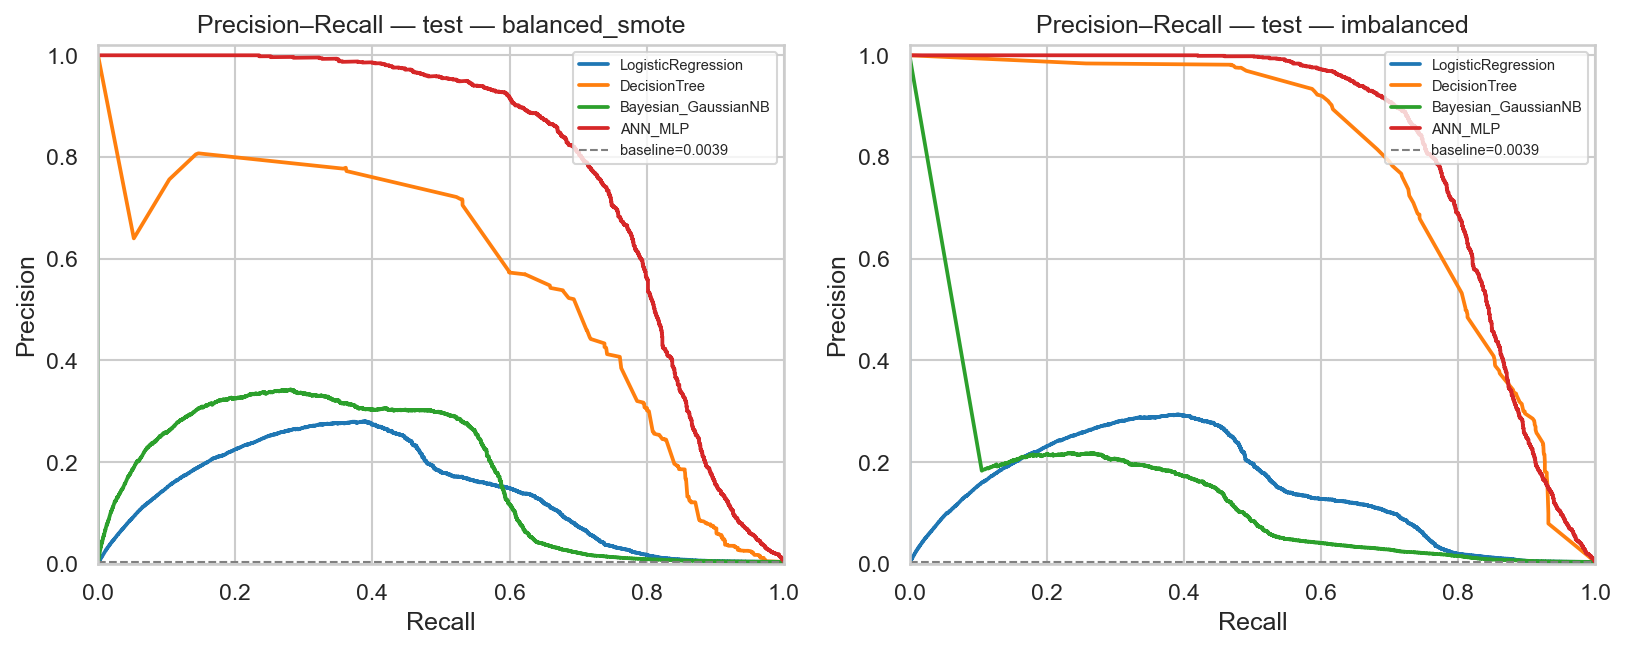
\includegraphics[width=1\textwidth]{Images/pr_test_threshold_0.5.png}
    \caption{Precision-Recall curve on test set}
    \label{fig:pr_test}
\end{figure}

\paragraph*{ROC Curves}

\begin{figure}[H]
    \centering
    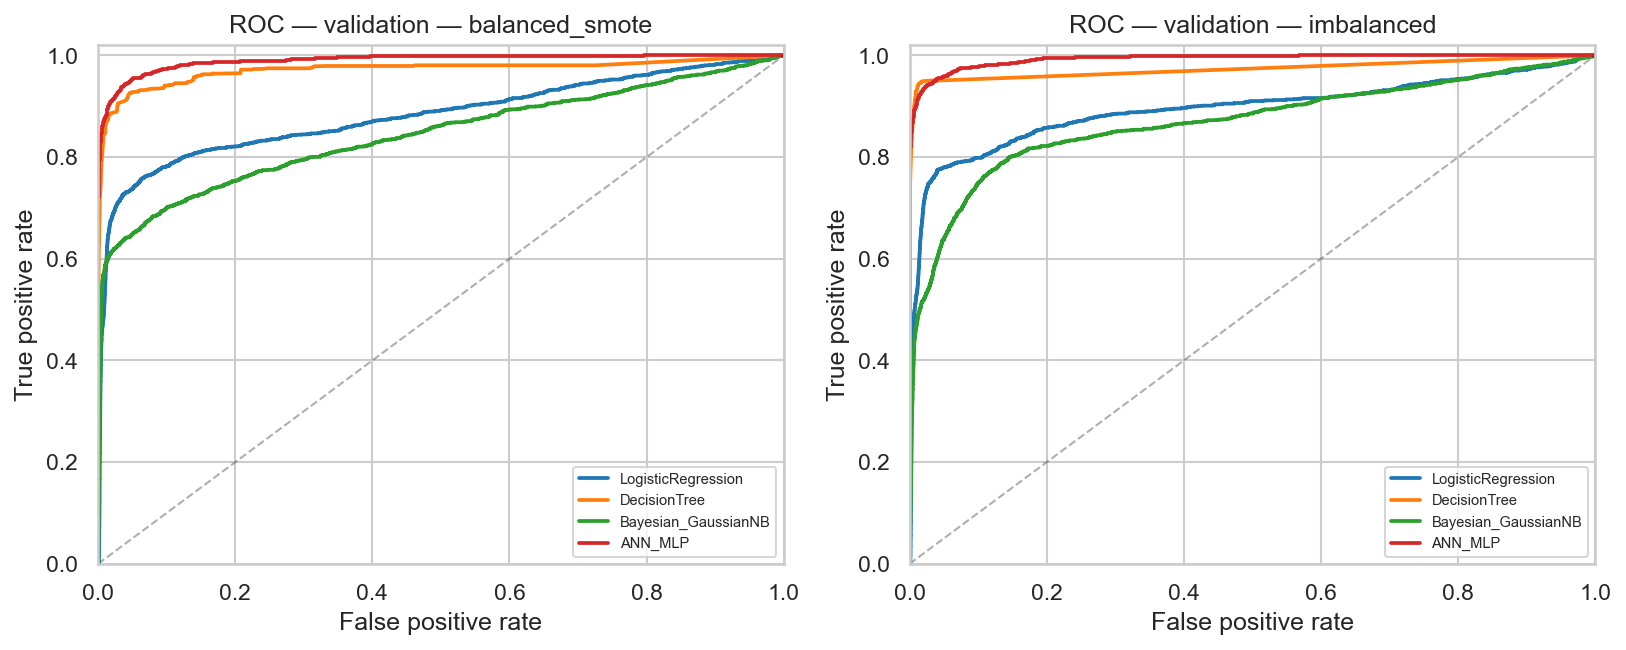
\includegraphics[width=1\textwidth]{Images/roc_valid_threshold_0.5.png}
    \caption{ROC curve on validation set}
    \label{fig:roc_valid}
\end{figure}

\begin{figure}[H]
    \centering
    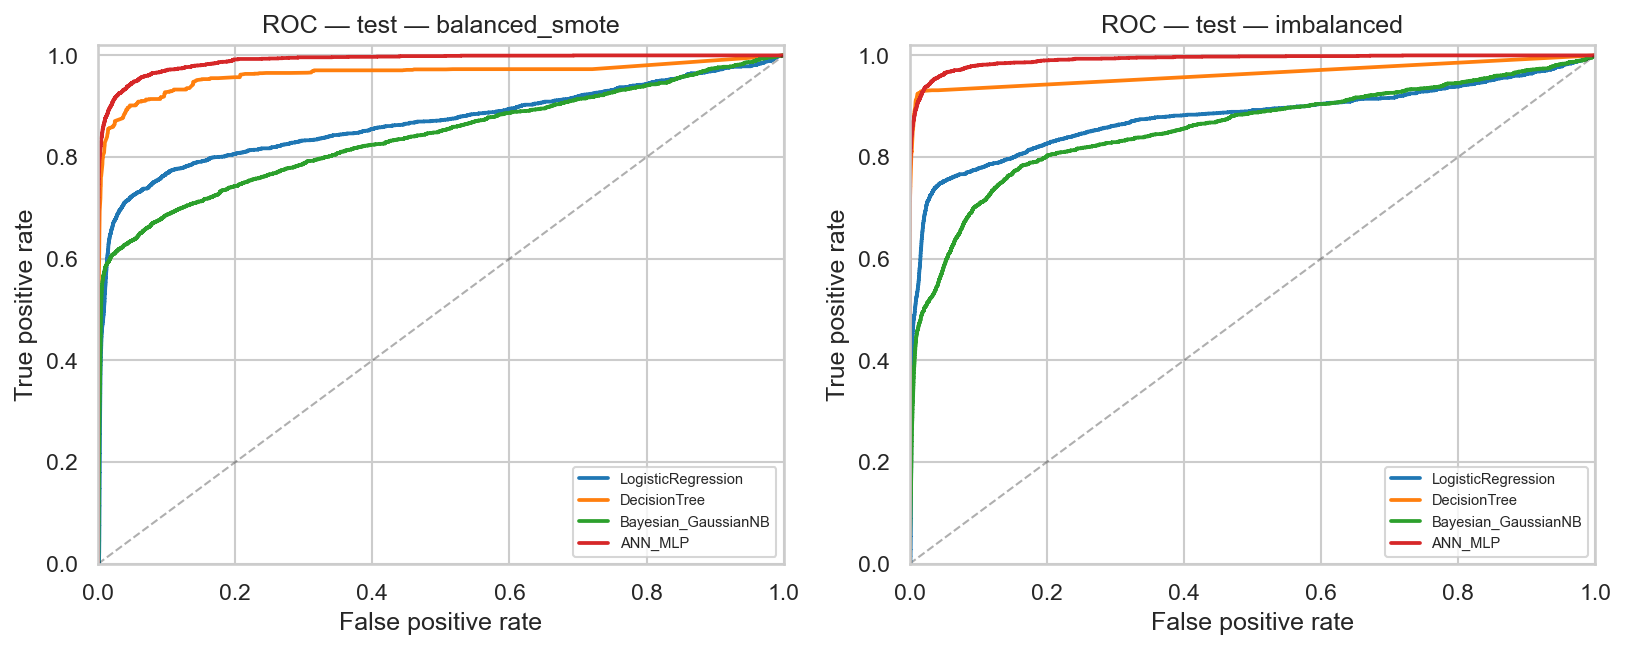
\includegraphics[width=1\textwidth]{Images/roc_test_threshold_0.5.png}
    \caption{ROC curve on test set}
    \label{fig:roc_test}
\end{figure}


\paragraph*{Analysis and Insights}

From the visualizations, several important observations can be drawn.

First, the metric comparison shows that the ANN model trained on the imbalanced dataset provides the best overall performance. It achieves a strong balance between Precision and Recall, resulting in the highest F1-score and PR-AUC among all models. In contrast, the Decision Tree model achieves the highest Recall, indicating its ability to detect most fraudulent transactions, but suffers from significantly lower Precision.

Second, the confusion matrices further highlight this trade-off. The Decision Tree produces a large number of false positives, which may lead to excessive false alarms in real-world applications. On the other hand, the ANN model maintains a relatively low number of false positives while still detecting a substantial portion of fraud cases, making it more practical for deployment.

Third, the Precision-Recall curves confirm that the ANN model consistently dominates other models across different recall levels. This indicates superior performance in handling the minority (fraud) class. Logistic Regression and Naive Bayes show noticeably weaker performance, especially at higher recall regions.

Finally, although ROC curves suggest that all models perform well with high ROC-AUC values, this metric can be overly optimistic for imbalanced datasets. In this context, PR-AUC provides a more reliable evaluation, and again, the ANN model demonstrates the best effectiveness.

Overall, the results indicate that the ANN model trained on the imbalanced dataset offers the most balanced and robust performance, while the Decision Tree model is more suitable in scenarios where maximizing fraud detection (Recall) is the highest priority.



\subsection{Discussion}

The experimental results reveal several important insights:

\begin{itemize}
    \item Increasing the threshold to $0.7$ improves \textbf{precision} but significantly reduces \textbf{recall}, meaning more fraud cases are missed.
    
    \item Reducing the threshold to $0.2$ dramatically improves \textbf{recall}, but at the cost of lower precision and accuracy. This leads to many false positives.
    
    \item Models trained on the \textbf{imbalanced dataset}, especially ANN, consistently achieve better overall balance (high precision, strong PR-AUC).
    
    \item \textbf{SMOTE} improves recall but often degrades overall model quality, particularly precision and stability.
    
    \item The \textbf{Decision Tree} achieves the highest recall across multiple settings, but suffers from low precision, making it less reliable in practice.
    
    \item The \textbf{ANN model} provides the most stable and balanced performance across all thresholds.
\end{itemize}



\subsection{Conclusion}

There are two main approaches for model selection:

\begin{itemize}
    \item \textbf{Balanced performance}: choose ANN (imbalanced, threshold $0.5$) for strong overall metrics, providing a good trade-off between Precision and Recall.
    
    \item \textbf{Fraud-sensitive detection}: 
    \begin{itemize}
        \item ANN (imbalanced, threshold $0.2$) offers high recall while maintaining reasonable Precision.
        \item Decision Tree (imbalanced) achieves the \textbf{highest recall}, making it suitable in scenarios where detecting as many fraud cases as possible is the top priority.
    \end{itemize}
\end{itemize}

In real-world banking systems, missing fraudulent transactions is often more costly than false alarms. Therefore, models with high recall are preferred.

However, the Decision Tree model produces a large number of false positives, which may lead to inefficiency in downstream review processes. In contrast, the ANN model maintains a better balance between detecting fraud and limiting false alarms.

Overall, the \textbf{ANN model trained on imbalanced data with threshold $0.2$} is considered the most suitable solution, as it achieves high recall while preserving a more practical balance in overall performance.